\mbox{}
\newpage 
%//------ Section 03 -------------------------------------------------------------------------------------------------
\chapter{Complementary materials for the analysis:\\Mass measurements of multi-strange baryons in pp collisions at \sqrtS = 13 TeV}
\label{appendix:CPTAnalysis}
%//-----------------------------------------------------------------------//

\newpage

\section{Study of the systematic effects: topological and track selections}

%\subsection{Topological and track selections}

\begin{table}[h]
    \centering
    \begin{tabular}{c|c|c}
    \noalign{\smallskip}\hline \noalign{\smallskip}
    \bf Candidate variable & Range & Signal variation \rmKzeroS \\
    \noalign{\smallskip}\hline \noalign{\smallskip}    
    Competing mass rejection (\gmass) & $> \left[ 0.002 ; 0.010 \right]$ & 1.1\% \\
    
    \noalign{\smallskip}\hline \noalign{\smallskip}
    \bf Track variable & Range & Signal variation \rmKzeroS \\
    \noalign{\smallskip}\hline \noalign{\smallskip}
    Nbr of crossed TPC readout rows & $> \left[ 70 ; 90 \right]$ &  0.5\% \\
    $\Nsigma^{\rm TPC}$ & $< \left[ 1 ; 3 \right] \ \sigma$ &  45\% \\
    
    \noalign{\smallskip}\hline \noalign{\smallskip}
    \bf Topological variable & Range & Signal variation \rmKzeroS \\
    \noalign{\smallskip}\hline \noalign{\smallskip}
    
    V0 decay radius (\cm) & $> \left[ 0.4 ; 2.2 \right]$ & 10\% \\
    V0 Lifetime (\cm) & $< \left[ 1.57 ; 3.43 \right]$ \cTau & 12\% \\
    V0 cosine of pointing angle & $> \left[ 0.995 ; 0.9998 \right]$ & 10\% \\
    DCA pion to prim. vtx (\cm) & $> \left[ 0.04 ; 0.5 \right]$ & 24\% \\
%    DCA V0 to prim. vtx (\cm) & < $\left[ 0.04 ; 1 \right]$ & 35\% \\
    DCA between V0 daughters (std dev) & $< \left[ 0.2 ; 1.5 \right]$ & 12\%\\
    \noalign{\smallskip}\hline \noalign{\smallskip}
    \end{tabular}
    \caption{Summary of the variation ranges on the topological and track selections used for the reconstruction of \rmKzeroS. The induced signal variation is indicated in the last column; for more details, look at \fig\ref{fig:SignalVariation_TopoSel_K0s}.}\label{tab:SystematicSelectionsK0s}
\end{table}

\begin{table}[h]
    \centering
    \begin{tabular}{c|c|c}
    \noalign{\smallskip}\hline \noalign{\smallskip}
    \bf Candidate variable & Range & Signal variation \rmLambda (\rmAlambda) \\
    \noalign{\smallskip}\hline \noalign{\smallskip}    
    Competing mass rejection (\gmass) & > $\left[ 0.005 ; 0.012 \right]$ & 3\% (3\%)\\
    
    \noalign{\smallskip}\hline \noalign{\smallskip}
    \bf Track variable & Range & Signal variation \rmLambda (\rmAlambda) \\
    \noalign{\smallskip}\hline \noalign{\smallskip}
    Nbr of crossed TPC readout rows & > $\left[ 70 ; 90 \right]$ &  0.8\% (0.8\%)\\
    $\Nsigma^{\rm TPC}$ & < $\left[ 1 ; 3 \right] \ \sigma$ &  45\% (45\%)\\
    
    \noalign{\smallskip}\hline \noalign{\smallskip}
    \bf Topological variable & Range & Signal variation \rmLambda (\rmAlambda) \\
    \noalign{\smallskip}\hline \noalign{\smallskip}
    
    V0 decay radius (\cm) & $> \left[ 0.4 ; 3.5 \right]$ & 11\% (11\%)\\
    V0 Lifetime (\cm) & $< \left[ 1.53 ; 3.43 \right]$ \cTau & 17\% (17\%)\\
    V0 cosine of pointing angle & $> \left[ 0.995 ; 0.9998 \right]$ & 13\% (13\%)\\
    DCA proton to prim. vtx (\cm) & $> \left[ 0.04 ; 0.15 \right]$ & 17\% (17\%)\\
    DCA pion to prim. vtx (\cm) & $> \left[ 0.04 ; 0.5 \right]$ & 12\% (12\%) \\
%    DCA V0 to prim. vtx (\cm) & $< \left[ 0.06 ; 0.2 \right]$ & 25\% (25\%)\\
    DCA between V0 daughters (std dev) & $< \left[ 0.3 ; 1.5 \right]$ & 12\% (12\%)\\ 
    \noalign{\smallskip}\hline \noalign{\smallskip}
    \end{tabular}
    \caption{Summary of the variation ranges on the topological and track selections used for the reconstruction of \rmLambda and \rmAlambda. The induced signal variation is indicated in the last column; for more details, look at \fig\ref{fig:SignalVariation_TopoSel_Lambda} and \fig\ref{fig:SignalVariation_TopoSel_AntiLambda}.}\label{tab:SystematicSelectionsLambda}
\end{table}

\begin{landscape}
\begin{figure}[h]
	\centering
	\includegraphics[width=1.45\textwidth]{Figs/Chapter5/SignalVariation\_XiMinus.eps}
\caption{Signal variation within the selection range of every topological and track variables used in the \rmXiM analysis. These distributions were obtained by fixing all the cuts to their values in \tab\ref{tab:CascadeSelections} but one;  the procedure in \Sec\ref{subsubsec:SystTopoMass} is then used to vary randomly the latter within its range of selections (see \tab\ref{tab:SystematicSelectionsXi}). The ratio between the extracted signal and the average signal within the selection range provides the signal variation. Here, the signal was computed based on the fit of the invariant mass using a modified Gaussian for the peak and a first order polynomial for the background.}
	\label{fig:SignalVariation_TopoSel_XiMinus}
\end{figure}

\begin{figure}[h]
	\centering
	\includegraphics[width=1.45\textwidth]{Figs/Chapter5/SignalVariation\_XiPlus.eps}
\caption{Signal variation within the selection range of every topological and track variables used in the \rmAxiP analysis. These distributions were obtained by fixing all the cuts to their values in \tab\ref{tab:CascadeSelections} but one; the procedure in \Sec\ref{subsubsec:SystTopoMass} is then used to vary randomly the latter within its range of selections (see \tab\ref{tab:SystematicSelectionsXi}). The ratio between the extracted signal and the average signal within the selection range provides the signal variation. Here, the signal was computed based on the fit of the invariant mass using a modified Gaussian for the peak and a first order polynomial for the background.}
	\label{fig:SignalVariation_TopoSel_XiPlus}
\end{figure}

\begin{figure}[h]
	\centering
	\includegraphics[width=1.45\textwidth]{Figs/Chapter5/SignalVariation\_OmegaMinus.eps}
\caption{Signal variation within the selection range of every topological and track variables used in the \rmOmegaM analysis. These distributions were obtained by fixing all the cuts to their values in \tab\ref{tab:CascadeSelections} but one; the procedure in \Sec\ref{subsubsec:SystTopoMass} is then used to vary randomly the latter within its range of selections (see \tab\ref{tab:SystematicSelectionsOmega}). The ratio between the extracted signal and the average signal within the selection range provides the signal variation. Here, the signal was computed based on the fit of the invariant mass using a modified Gaussian for the peak and a first order polynomial for the background.}
	\label{fig:SignalVariation_TopoSel_OmegaMinus}
\end{figure}

\begin{figure}[h]
	\centering
	\includegraphics[width=1.45\textwidth]{Figs/Chapter5/SignalVariation\_OmegaPlus.eps}
\caption{Signal variation within the selection range of every topological and track variables used in the \rmAomegaP analysis. These distributions were obtained by fixing all the cuts to their values in \tab\ref{tab:CascadeSelections} but one; the procedure in \Sec\ref{subsubsec:SystTopoMass} is then used to vary randomly the latter within its range of selections (see \tab\ref{tab:SystematicSelectionsOmega}). The ratio between the extracted signal and the average signal within the selection range provides the signal variation. Here, the signal was computed based on the fit of the invariant mass using a modified Gaussian for the peak and a first order polynomial for the background.}
	\label{fig:SignalVariation_TopoSel_OmegaPlus}
\end{figure}

\begin{figure}[h]
	\centering
	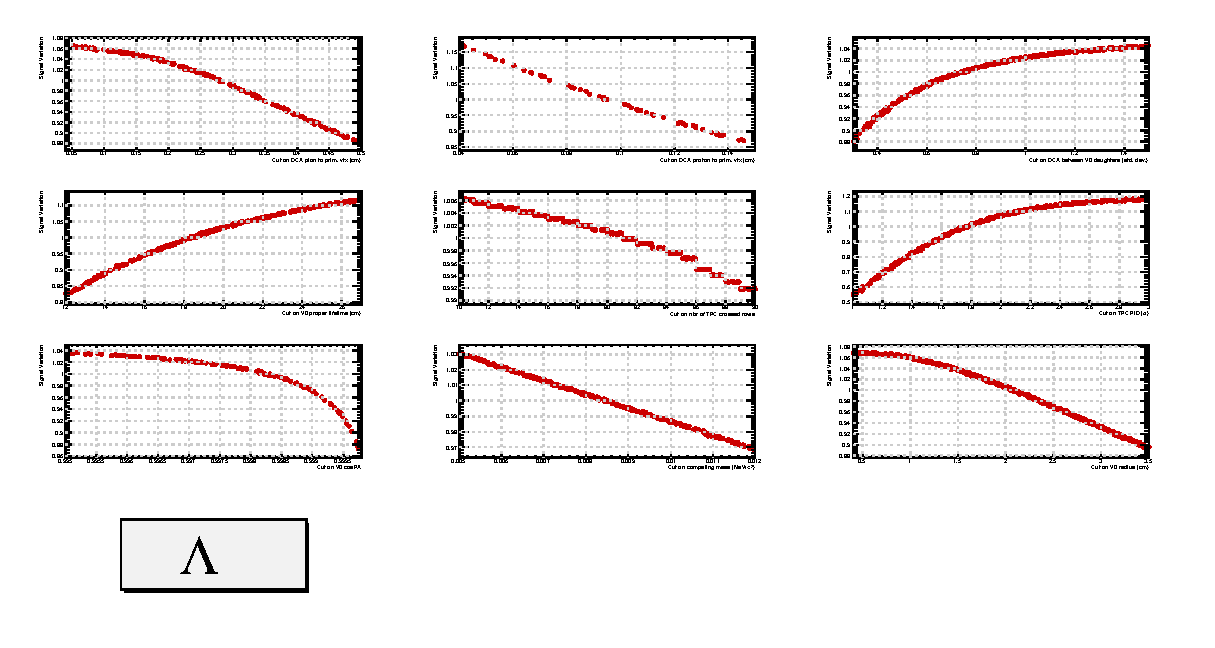
\includegraphics[width=1.45\textwidth]{Figs/Chapter5/SignalVariation_Lambda.eps}
\caption{Signal variation within the selection range of every topological and track variables used in the \rmLambda analysis. These distributions were obtained by fixing all the cuts to their values in \tab\ref{tab:V0Selections} but one; the procedure in \Sec\ref{subsubsec:SystTopoMass} is then used to vary randomly the latter within its range of selections (see \tab\ref{tab:SystematicSelectionsLambda}). The ratio between the extracted signal and the average signal within the selection range provides the signal variation. Here, the signal was computed based on the fit of the invariant mass using a modified Gaussian for the peak and a first order polynomial for the background.}
	\label{fig:SignalVariation_TopoSel_Lambda}
\end{figure}

\begin{figure}[h]
	\centering
	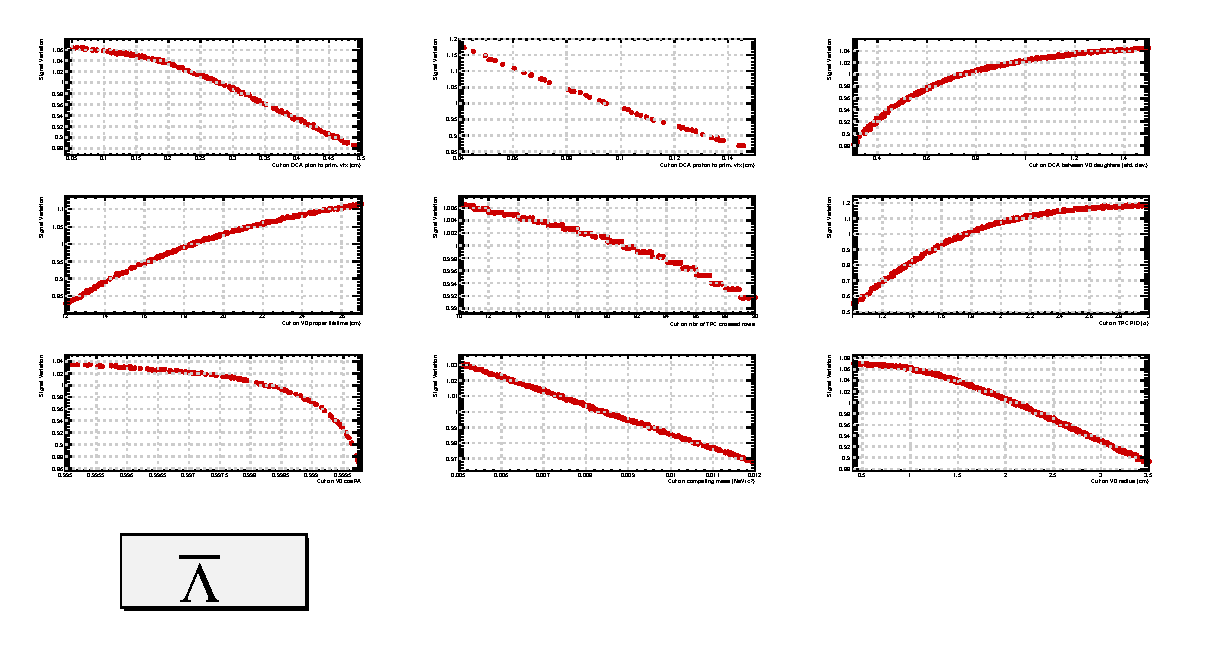
\includegraphics[width=1.45\textwidth]{Figs/Chapter5/SignalVariation_AntiLambda.eps}
\caption{Signal variation within the selection range of every topological and track variables used in the \rmAlambda analysis. These distributions were obtained by fixing all the cuts to their values in \tab\ref{tab:V0Selections} but one; the procedure in \Sec\ref{subsubsec:SystTopoMass} is then used to vary randomly the latter within its range of selections (see \tab\ref{tab:SystematicSelectionsLambda}). The ratio between the extracted signal and the average signal within the selection range provides the signal variation. Here, the signal was computed based on the fit of the invariant mass using a modified Gaussian for the peak and a first order polynomial for the background.}
	\label{fig:SignalVariation_TopoSel_AntiLambda}
\end{figure}

\begin{figure}[h]
	\centering
	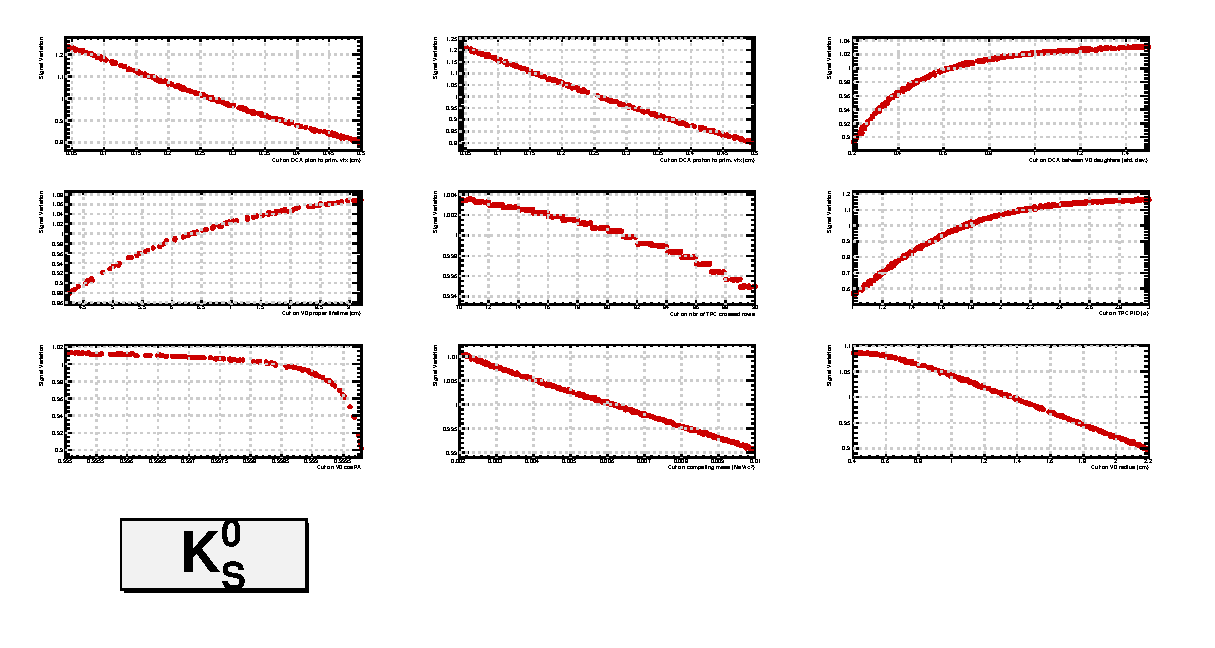
\includegraphics[width=1.45\textwidth]{Figs/Chapter5/SignalVariation_K0s.eps}
\caption{Signal variation within the selection range of every topological and track variables used in the \rmKzero analysis. These distributions were obtained by fixing all the cuts to their values in \tab\ref{tab:V0Selections} but one; the procedure in \Sec\ref{subsubsec:SystTopoMass} is then used to vary randomly the latter within its range of selections (see \tab\ref{tab:SystematicSelectionsK0s}). The ratio between the extracted signal and the average signal within the selection range provides the signal variation. Here, the signal was computed based on the fit of the invariant mass using a modified Gaussian for the peak and a first order polynomial for the background.}
	\label{fig:SignalVariation_TopoSel_K0s}
\end{figure}
\end{landscape}

\section{Summary of the systematic uncertainties}
\label{sec:SummarySystUncertaintiesV0s}

\begin{table}[H]
    \centering
    \begin{tabular}{c|c|c}
    \noalign{\smallskip}\hline \noalign{\smallskip}
    \bf  & \multicolumn{2}{c}{Uncertainties on the measured mass (\mmass)} \\
    \bf Sources & \multicolumn{2}{c}{\rmKzeroS}\\
    \bf  & Statistical & Systematic \\
    \noalign{\smallskip}\hline \noalign{\smallskip}
    Topological selections & 0.022 & 0.013 \\
    Momentum calibration & / & 0.229\\
    Magnetic field & / & 0.080 \\
    Material budget & / & 0.052\\
    Fitting function & / & 0.006 \\
    Fitting range & / & 0.001 \\    
    Binning & / & 0.001\\
    Out-of-bunch pile-up rejection & / & 0.029 \\
    Precision on the PDG mass & / & negligible\\
    MC mass offset & / & 0.047\\
    \noalign{\smallskip}\hline \noalign{\smallskip}
    \bf Total &\bf 0.022 &\bf 0.256\\
    \noalign{\smallskip}\hline \noalign{\smallskip}
    \end{tabular}
    \caption{Statistical and systematic uncertainties on the mass \rmKzeroS. The total is obtained assuming that there is no correlation between each source of uncertainties.}\label{tab:SystMassK0s}
\end{table}

\begin{table}[H]
    \centering
    \begin{tabular}{c|c|c|c|c}
    \noalign{\smallskip}\hline \noalign{\smallskip}
    \bf  & \multicolumn{4}{c}{Uncertainties on the measured mass (\mmass)} \\
    \bf Sources & \multicolumn{2}{c|}{\rmLambda} & \multicolumn{2}{c}{\rmAlambda}\\
    \bf  & Statistical & Systematic & Statistical & Systematic\\
    \noalign{\smallskip}\hline \noalign{\smallskip}
    Topological selections & 0.011 & 0.006 & 0.011 & 0.004\\
    Momentum calibration & / & 0.056 & / & 0.056 \\
    Magnetic field & / & 0.013 & / & 0.013 \\
    Material budget & / & 0.020 & / & 0.020 \\
    Fitting function & / & 0.009 & / & 0.009\\
    Fitting range & / & 0.001 & / & 0.001 \\    
    Binning & / & 0.001 & / & 0.001 \\
    Out-of-bunch pile-up rejection & / & 0.004 & / & 0.004 \\
    Precision on the PDG mass & / & negligible & / & negligible \\
    MC mass offset & / & 0.015 & / & 0.015 \\
    \noalign{\smallskip}\hline \noalign{\smallskip}
    \bf Total &\bf 0.011 &\bf 0.066 &\bf 0.011 &\bf 0.065 \\
    \noalign{\smallskip}\hline \noalign{\smallskip}
    \end{tabular}
    \caption{Statistical and systematic uncertainties on the mass \rmLambda and \rmAlambda. The total is obtained assuming that there is no correlation between each source of uncertainties.}\label{tab:SystMassLambda}
\end{table}

\begin{table}[H]
    \centering
    \begin{tabular}{c|c|c}
    \noalign{\smallskip}\hline \noalign{\smallskip}
    \bf  & \multicolumn{2}{c}{Uncertainties on the measured mass difference ($\times 10^{-5}$)} \\
    \bf Sources & \multicolumn{2}{c}{\rmLambda} \\
    \bf  & Statistical & Systematic \\
    \noalign{\smallskip}\hline \noalign{\smallskip}
    Topological selections & 1.34 & 1.31\\
    Momentum calibration & / & negligible \\
    Magnetic field & / & negligible \\
    Material budget & / & negligible\\
    Fitting function & / & 0.69\\
    Fitting range & / & 0.02 \\    
    Binning & / & 0.02 \\
    Out-of-bunch pile-up rejection & / & negligible\\
    Precision on the PDG mass & / & negligible\\
    MC mass offset & / & 1.72 \\
    \noalign{\smallskip}\hline \noalign{\smallskip}
    \bf Total &\bf 1.34 & \bf 2.27 \\
    \noalign{\smallskip}\hline \noalign{\smallskip}
    \end{tabular}
    \caption{Statistical and systematic uncertainties on the mass \rmLambda and \rmAlambda. The total is obtained assuming that there is no correlation between each source of uncertainties.}\label{tab:SystMassDiffLambda}
\end{table}

\section{Discussion}
\label{appendix:DiscussionCPT}

In its listings, the PDG \cite{particledatagroupReviewParticlePhysics2022} provides several values for a given quantity. Concerning the mass and mass difference of multi-strange baryons, two kind of values are usually specified:

\begin{itemize}
\item[$\bullet$] the \textbf{PDG average} or world average which corresponds to the weighted average of the selected data,
\item[$\bullet$] and the \textbf{PDG fit}, which coincides with the so-called \say{PDG value} used by everyone and is obtained from a constrained multi-parameter fit of the selected data.
\end{itemize}

Throughout this manuscript, the term \say{PDG value} refers to the latter value. There can be some exceptions, such as mass and mass difference values for the \rmXiPM hyperons. In such case, only the latest measurement is considered. Consequently, the \textit{PDG average} is in fact the measured value quoted in the publication, while the \textit{PDG fit} consists in a fit considering only the measured values for the particle and the anti-particle.\\

As a comparison, we provide the world averages including our measurements for the mass and mass difference of \rmXiPM and \rmOmegaPM baryons. The numerical values can be found in \tab\ref{tab:FinalResultsCPTWorldAvg}, and the comparisons to past measurements are displayed in \figs\ref{fig:MassWorldAvgVsPDG} and \ref{fig:MassDiffWorldAvgVsPDG}.

\begin{table}[h]
%    \hspace{-1.3cm}
	\centering
    \begin{tabular}{c|c|c|c}

%    \begin{tabular}{b{2cm}@{\hspace{0.5cm}} b{3cm}@{\hspace{0.5cm}} b{2cm}@{\hspace{0.5cm}} b{2cm}@{\hspace{0.5cm}} b{5cm}@{\hspace{0.5cm}} b{3cm}@{\hspace{0.5cm}} b{3cm}@{\hspace{0.5cm}}}
    \noalign{\smallskip}\hline \noalign{\smallskip}
    \bf Particle & \bf PDG average & \bf PDG fit & \bf Our world average\\
    & (\mmass) & (\mmass) & (\mmass) \\
    \noalign{\smallskip}\hline \noalign{\smallskip}
    \rmXiM & 1321.70 $\pm$ 0.10 & 1321.71 $\pm$ 0.07 & 1321.792 $\pm$ 0.056\\
	\rmAxiP & 1321.73 $\pm$ 0.10 & 1321.71 $\pm$ 0.07 & 1321.823 $\pm$ 0.062 \\
    \noalign{\smallskip}\hline \noalign{\smallskip}
    \rmOmegaM & 1672.43 $\pm$ 0.32 & 1672.45 $\pm$ 0.29 & 1672.512 $\pm$ 0.103\\ 
    \rmAomegaP & 1672.5 $\pm$ 0.7 & 1672.45 $\pm$ 0.29 & 1672.509 $\pm$ 0.100\\ 
	\noalign{\smallskip}\hline \noalign{\smallskip}
	\bf Particle & \bf PDG value & \bf Our value & \bf Our world average\\
    & ($\times 10^{-5}$) & ($\times 10^{-5}$) & ($\times 10^{-5}$) \\
    \noalign{\smallskip}\hline \noalign{\smallskip}
    \rmXi & 2.5 $\pm$ 8.7 & -3.34 $\pm$ 7.13 & -1.00 $\pm$ 5.52 \\
    \noalign{\smallskip}\hline \noalign{\smallskip}
    \rmOmega & 1.44 $\pm$ 7.98 & 3.44 $\pm$ 3.92 & 3.06 $\pm$ 3.52\\ 
	\noalign{\smallskip}\hline \noalign{\smallskip}
    \end{tabular}
    \caption{Top: the PDG average, PDG fit and the world average value including our measured masses, with their total uncertainties, for \rmXiPM and \rmOmegaPM baryons. Bottom: PDG value, our measured mass difference and our world average value including our measured mass differences, with their total uncertainties, for \rmXi and \rmOmega baryons. Here, the PDG value corresponds in fact to the latest measurement \cite{abdallahMassesLifetimesProduction2006, chanMeasurementPropertiesOverline1998}.}\label{tab:FinalResultsCPTWorldAvg}
\end{table}

\begin{figure}[h]
%\centering
\hspace*{-2cm}
\subfigure[]{
	\includegraphics[width=0.6\textwidth]{Figs/Chapter5/MassXiMinus\_New\_WorldAvg.eps}
	\label{fig:MassXiMinusWorldAvgVsPDG}
} 
\subfigure[]{
	\includegraphics[width=0.6\textwidth]{Figs/Chapter5/MassXiPlus\_New\_WorldAvg.eps}
	\label{fig:MassXiPlusWorldAvgVsPDG}
}
\hspace*{-2cm}
\subfigure[]{
	\includegraphics[width=0.6\textwidth]{Figs/Chapter5/MassOmegaMinus\_New\_WorldAvg.eps}
	\label{fig:MassOmegaMinusWorldAvgVsPDG}
} 
\subfigure[]{
	\includegraphics[width=0.6\textwidth]{Figs/Chapter5/MassOmegaPlus\_New\_WorldAvg.eps}
	\label{fig:MassOmegaPlusWorldAvgVsPDG}
}
\caption{Comparison of our mass values for the \rmXiM (a), \rmAxiP (b), \rmOmegaM (c) and \rmAomegaP (d) hyperons, to the past measurements quoted in the PDG, as of 2023 \cite{particledatagroupReviewParticlePhysics2022}. The vertical line and the shaded area in blue represent the PDG value and its associated uncertainty, while those in orange correspond to the world average including our measurement and its associated uncertainties.}
	\label{fig:MassWorldAvgVsPDG}
\end{figure}

\begin{figure}[h]
%\centering
\hspace*{-2cm}
\subfigure[]{
	\includegraphics[width=0.6\textwidth]{Figs/Chapter5/MassDiff\_Xi\_New\_WorldAvg.eps}
	\label{fig:MassDiffXiWorldAvgVsPDG}
} 
\subfigure[]{
	\includegraphics[width=0.6\textwidth]{Figs/Chapter5/MassDiff\_Omega\_New\_WorldAvg.eps}
	\label{fig:MassDiffOmegaWorldAvgVsPDG}
}
\caption{Comparison of our mass difference values between the \rmXiM and \rmAxiP (a), and the \rmOmegaM and \rmAomegaP, to the past measurements quoted in the PDG, as of 2023 \cite{particledatagroupReviewParticlePhysics2022}. The vertical line and the shaded area in blue represent the PDG value and its associated uncertainty, while those in orange correspond to the world average including our measurement and its associated uncertainties.}
	\label{fig:MassDiffWorldAvgVsPDG}
\end{figure}

%\begin{table}[p]
%    \centering
%    \begin{tabular}{c|c|c|c|c}
%    \noalign{\smallskip}\hline \noalign{\smallskip}
%    \bf  & \multicolumn{4}{c}{Systematic uncertainties} \\
%    \bf Sources & \multicolumn{4}{c}{On the measured mass (\mmass)} \\
%    \bf & \rmXiM & \rmAxiP & \rmOmegaM & \rmAomegaP \\
%    \noalign{\smallskip}\hline \noalign{\smallskip}
%    Topological selections & 0.024 & 0.028 & 0.026 & 0.034 \\
%    Momentum calibration & negl. & negl. & 0.084 & 0.081\\
%    Magnetic field & 0.023 & 0.028 & 0.026 & 0.027\\
%    Material budget & 0.022 & 0.022 & 0.031 & 0.031\\
%    Fitting function & 0.009 & 0.009 & 0.007 & 0.007 \\
%    Fitting range & 0.001 & 0.001 & 0.001 & 0.001\\    
%    Binning & 0.001 & 0.001 & 0.001 & 0.001 \\
%    Out-of-bunch pile-up rejection & 0.006 & 0.006 & 0.004 & 0.003\\
%    Precision on the PDG mass & 0.011 & 0.011 & 0.018 & 0.018\\
%    MC mass offset & 0.055 & 0.058 & 0.021 & 0.019\\
%    \noalign{\smallskip}\hline \noalign{\smallskip}
%    \bf Total &\bf 0.075 &\bf 0.079 & \bf 0.102 & \bf 0.101\\
%    \noalign{\smallskip}\hline \noalign{\smallskip}
%    \end{tabular}
%    \caption{Statistical and systematical uncertainties on the mass \rmXiM and \rmAxiP. The total is obtained assuming that there is no correlation between each source of uncertainties.}
%\end{table}
%
%\begin{table}[p]
%    \hspace*{-0.5cm}
%    \begin{tabular}{c|c|c}
%    \noalign{\smallskip}\hline \noalign{\smallskip}
%    \bf  & \multicolumn{2}{c}{Uncertainties on the measured mass difference ($\times 10^{-5}$)} \\
%    \bf Sources & \multicolumn{2}{c}{\rmXi} \\
%    \bf  & Statistical & Systematic \\
%    \noalign{\smallskip}\hline \noalign{\smallskip}
%    Topological selections & 2.77 & 4.27\\
%    Momentum calibration & / & negligible \\
%    Magnetic field & / & negligible \\
%    Material budget & / & negligible\\
%    Fitting function & / & 0.77\\
%    Fitting range & / & 0.03 \\    
%    Binning & / & 0.03 \\
%    Out-of-bunch pile-up rejection & / & negligible \\
%    Precision on the PDG mass & / & negligible\\
%    MC mass offset & / & 4.37 \\
%    \noalign{\smallskip}\hline \noalign{\smallskip}
%    \bf Total &\bf 2.77 &\bf 6.16 \\
%    \noalign{\smallskip}\hline \noalign{\smallskip}
%    \end{tabular}
%    \caption{Statistical and systematic uncertainties on the mass difference between \rmXiM and \rmAxiP. The total is obtained assuming that there is no correlation between each source of uncertainties.}\label{tab:SystMassDiffXi}
%\end{table}
%
%\begin{table}[p]
%    \hspace*{-0.5cm}
%    \begin{tabular}{c|c|c}
%    \noalign{\smallskip}\hline \noalign{\smallskip}
%    \bf  & \multicolumn{2}{c}{Uncertainties on the measured mass difference ($\times 10^{-5}$)} \\
%    \bf Sources & \multicolumn{2}{c}{\rmOmega} \\
%    \bf  & Statistical & Systematic \\
%    \noalign{\smallskip}\hline \noalign{\smallskip}
%    Topological selections & 2.94 & 1.63 \\
%    Momentum calibration & / & negligible \\
%    Magnetic field & / & negligible \\
%    Material budget & / & negligible\\
%    Fitting function & / & 0.28 \\
%    Fitting range & / & 0.03\\    
%    Binning & / & 0.13 \\
%    Out-of-bunch pile-up rejection & / & negligible\\
%    Precision on the PDG mass & / & negligible\\
%    MC mass offset & / & 1.70 \\
%    \noalign{\smallskip}\hline \noalign{\smallskip}
%    \bf Total &\bf 2.94 &\bf 2.38 \\
%    \noalign{\smallskip}\hline \noalign{\smallskip}
%    \end{tabular}
%    \caption{Statistical and systematic uncertainties on the mass difference between \rmOmegaM and \rmAomegaP. The total is obtained assuming that there is no correlation between each source of uncertainties.}\label{tab:SystMassDiffOmega}
%\end{table}
%
%\begin{table}[h]
%    \hspace{-1.3cm}
%    \begin{tabular}{cccc|ccc}
%
%%    \begin{tabular}{b{2cm}@{\hspace{0.5cm}} b{3cm}@{\hspace{0.5cm}} b{2cm}@{\hspace{0.5cm}} b{2cm}@{\hspace{0.5cm}} b{5cm}@{\hspace{0.5cm}} b{3cm}@{\hspace{0.5cm}} b{3cm}@{\hspace{0.5cm}}}
%    \noalign{\smallskip}\hline \noalign{\smallskip}
%    \bf Particle & \bf Measured & \multicolumn{2}{c|}{\bf Uncertainty} & \bf Previous & \multicolumn{2}{c}{\bf Uncertainty}\\
%    & \bf mass & \bf stat. & \bf syst. & \bf measured mass & \bf stat. & \bf syst.\\
%    & (\mmass) & (\mmass) & (\mmass) & (\mass) & (\mmass) & (\mass) \\
%    \noalign{\smallskip}\hline \noalign{\smallskip}
%    \rmXiM & 1321.975 & 0.026 & 0.075 & 1321.70 & 0.08 & 0.05 \\
%	\rmAxiP & 1321.988 & 0.024 & 0.079 & 1321.73 & 0.08 & 0.05 \\
%    \noalign{\smallskip}\hline \noalign{\smallskip}
%    \rmOmegaM & 1672.518 & 0.033 & 0.102 & 1673 & \multicolumn{2}{c}{1} \\ 
%    \rmAomegaP & 1672.563 & 0.033 & 0.101 & 1673 & \multicolumn{2}{c}{1} \\ 
%	\noalign{\smallskip}\hline \noalign{\smallskip}
%	\bf Particle & \bf Measured & \multicolumn{2}{c|}{\bf Uncertainty} & \bf Previous & \multicolumn{2}{c}{\bf Total}\\
%    & \bf mass difference & \bf stat. & \bf syst. & \bf mass difference & \multicolumn{2}{c}{\bf uncertainty} \\
%    & ($\times 10^{-5}$) & ($\times 10^{-5}$) & ($\times 10^{-5}$) & ($\times 10^{-5}$) & \multicolumn{2}{c}{($\times 10^{-5}$)}\\
%    \noalign{\smallskip}\hline \noalign{\smallskip}
%    \rmXi & -1.45 & 2.77 & 6.61 & 2.5 & \multicolumn{2}{c}{8.7} \\
%    \noalign{\smallskip}\hline \noalign{\smallskip}
%    \rmOmega & 3.21 & 2.94 & 2.38 & 1.44 & \multicolumn{2}{c}{7.98}\\ 
%	\noalign{\smallskip}\hline \noalign{\smallskip}
%    \end{tabular}
%    \caption{On the left: final measured masses and relative mass differences for \rmXiPM and \rmOmegaPM, with their associated statistical and systematic uncertainties. On the right: previous measurements of the mass and relative mass difference for the \rmXiPM \cite{abdallahMassesLifetimesProduction2006} and \rmOmegaPM \cite{hartouniInclusiveProductionEnsuremath1985}\cite{chanMeasurementPropertiesOverline1998}, with their statistical and systematic uncertainties. If these values are not quoted in the paper, the total uncertainty is indicated.}\label{tab:FinalResultsCPT}
%\end{table}

%
%
%\begin{table}[p]
%%    \centering
%\hspace*{-2cm}
%    \begin{tabular}{c|c|c|c|c|c}
%    \noalign{\smallskip}\hline \noalign{\smallskip}
%    \bf \bf Particle & \bf Data & \bf Correlation & \multicolumn{3}{c}{\bf Comparison to MC models}\\
%    \bf Pair & \bf Sample & \bf Measurement & \Pythiaeight \textsc{Monash 2013} & \Pythiaeight \textsc{Colour Rope} & \EposFour\\
%    \noalign{\smallskip}\hline \noalign{\smallskip}
%    \multirow{2}*{\rmXiPM-\rmPhiMes} & MB & \CheckGr & \CheckGr & \CheckGr & \CheckGr \\
%     & HM & \CheckGr & \NoWay & \NoWay & \NoWay \\
%    \noalign{\smallskip}\hline \noalign{\smallskip}
%    \multirow{2}*{\rmOmegaPM-\rmPhiMes} & MB & \NoWay & \CheckGr & \CheckGr & \CheckGr \\
%     & HM & \CheckGr & \NoWay & \NoWay & \NoWay \\
%    \noalign{\smallskip}\hline \noalign{\smallskip}
%    \end{tabular}
%    \caption{Statistical and systematical uncertainties on the mass \rmXiM and \rmAxiP. The total is obtained assuming that there is no correlation between each source of uncertainties.}
%\end{table}
